\documentclass{article}
\usepackage[utf8]{inputenc}
\usepackage[fontsize=13pt]{scrextend}
\usepackage{geometry}
\usepackage{multicol}
\usepackage{xeCJK} 
\usepackage{lmodern} % For scalable Computer Modern fonts
\usepackage[T1]{fontenc} % Ensures proper font encoding
\usepackage{color}
\usepackage{helvet}  % For changing fonts

\usepackage{soul}  % For highlighting

\geometry{
  a4paper,
  left=25mm,
  right=25mm,
  top=25mm,
  bottom=25mm,
  heightrounded,
}

\documentclass{article}
\usepackage[utf8]{inputenc}
\usepackage[T1]{fontenc}
\usepackage{lmodern}
\usepackage{booktabs}
\usepackage{xcolor}
\usepackage{tikz}
\usepackage{pgfplots}
\usepackage{graphicx}

\usepackage{amsmath}


\usepackage{amsfonts}
\usepackage{amssymb}

\usepackage{tabularx}



\usepackage{hyperref}
\usepackage{listings}
\usepackage{booktabs}
\usepackage{tabularray}
\usepackage{multirow}
\usepackage{float}
\usepackage{lastpage}
\usepackage{tcolorbox}
\usepackage{titlesec}

\usepackage{etoolbox}

\makeatletter
\patchcmd{\@zfancyhead}{\fancy@reset}{\f@nch@reset}{}{}
\patchcmd{\@set@em@up}{\f@ncyolh}{\f@nch@olh}{}{}
\patchcmd{\@set@em@up}{\f@ncyolh}{\f@nch@olh}{}{}
\patchcmd{\@set@em@up}{\f@ncyorh}{\f@nch@orh}{}{}
\makeatother

\input{structure.tex}

\pgfplotsset{compat=newest}

% Colors from structure.tex
\definecolor{secondaryColor}{RGB}{0,0,0}
\definecolor{accentColor1}{RGB}{255,87,34}
\definecolor{accentColor3}{RGB}{63,81,181}
\definecolor{textColor}{RGB}{33,33,33}
\definecolor{primaryColor}{RGB}{34, 45, 101}
\definecolor{accentColor2}{RGB}{46, 117, 182}
\definecolor{backgroundColor}{RGB}{245, 245, 245}
\definecolor{fitcolor}{RGB}{0,128,0}
\definecolor{okaycolor}{RGB}{255,165,0}
\definecolor{notfitcolor}{RGB}{255,0,0}



\definecolor{sectioncolor}{RGB}{0,0,100}  % Deep blue for main headings
\definecolor{subcolor}{RGB}{100,0,100}  % Purple for subheadings
\definecolor{lightRed}{RGB}{255,200,200}  % Light red for section underline
\definecolor{lightPink}{RGB}{255,220,220}  % Light pink for subsection underline


\newcommand{\highlight}[1]{\textsf{\textbf{#1}}}  % For highlighting key terms in sans-serif bold
% Custom underline command
\newcommand{\customunderline}[2]{%
  \par\noindent\rule{0pt}{2ex}\vspace{-0.5in} % Adjust the space here
  \colorbox{#1}{\makebox[\linewidth]{#2}}\par
}

% Section format
\titleformat{\section}
  {\color{sectioncolor}\Huge\bfseries\sffamily}  % Sans-serif, huge, bold, blue
  {}
  {0pt}
  {}
  
 

% Subsection format
\titleformat{\subsection}
  {\color{subcolor}\Large\bfseries\sffamily}  % Sans-serif, large, bold, purple
  {}
  {0pt}
  {}

% % Adjust spacing
% \titlespacing*{\section}{0pt}{3.5ex plus 1ex minus .2ex}{2.3ex plus .2ex}
% \titlespacing*{\subsection}{0pt}{3.25ex plus 1ex minus .2ex}{1.5ex plus .2ex}


% % Modify the question environment to include color
% \renewenvironment{question}{
%   \vspace{0.5\baselineskip}
%   \section{}
%   \lfoot{\small\itshape\color{primaryColor}\assignmentQuestionName~\thesection~continued on next page\ldots}
% }{
%   \lfoot{}
% }

% Modify the answer command to include color
\renewcommand{\answer}[1]{
  \begin{tcolorbox}[
    breakable,
    enhanced,
    colback=backgroundColor,
    colframe=primaryColor,
    coltitle=white,
    title=Answer
  ]
    #1
  \end{tcolorbox}
}

% Modify the assignmentSection command to include color
\renewcommand{\assignmentSection}[1]{
  {
    \centering
    \vspace{2\baselineskip}
    
    \color{primaryColor}\rule{0.8\textwidth}{0.5pt}
    
    \vspace{0.75\baselineskip}
    {\LARGE\color{primaryColor}\MakeUppercase{#1}}
    
    \color{primaryColor}\rule{0.8\textwidth}{0.5pt}
    
    \vspace{\baselineskip}
  }
}

% Modify headers and footers to include color
\lhead{\small\color{primaryColor}\assignmentClass\ifdef{\assignmentClassInstructor}{\ (\assignmentClassInstructor):}{Ayush Kumar Mishra}\ \assignmentTitle}
\rhead{\small\color{secondaryColor}\ifdef{\assignmentAuthorName}{\assignmentAuthorName}{\ifdef{\assignmentDueDate}{Due\ \assignmentDueDate}{}}}
\cfoot{\small\color{primaryColor}Page\ \thepage\ of\ \pageref{LastPage}}

\renewcommand\headrulewidth{0.5pt}
\renewcommand{\headrule}{\hbox to\headwidth{\color{primaryColor}\leaders\hrule height \headrulewidth\hfill}}

\hypersetup{
    colorlinks=true,
    linkcolor=primaryColor,
    filecolor=accentColor1,      
    urlcolor=accentColor3,
    pdftitle={Advanced EDA of Video Text Dataset},
    pdfpagemode=FullScreen,
}

\title{\textcolor{primaryColor}{\Huge\textbf{EDA Analysis}}}
\author{\textcolor{secondaryColor}{\Large Ayush Kumar Mishra}}
\date{\textcolor{secondaryColor}{\today}}

\begin{document}

\maketitle

\newpage
\section*{Dashboard}
  \begin{center}
        \color{red}\rule{1\linewidth}{1mm}
    \end{center}
\begin{center}
\vspace{2in}
    {\Huge  For seeing all the code live interactively, \\
    \vspace{2in}
    Visit  \href{https://eda-analysis-iby-0.streamlit.app/}{Dashboard}}\\
    
    \vspace{0.7in}
   \textbf{ \href{https://eda-analysis-iby-0.streamlit.app/}{https://eda-analysis-iby-0.streamlit.app/}}
\end{center}

\newpage
\tableofcontents



\newpage
\large

After all the preprocessing and cleaning of the data, I have created a new dataframe which contains the average scores of all the features for each student.\\
I have explained this process in main.pdf file.\\
So this is my new DATAFRAME , Let's call it \textsc{final\_df}


\begin{tcolorbox}[colback=blue!5!white, colframe=green!70!black, title=Final Dataframe, fonttitle=\bfseries\Large]
    \begin{tblr}{
        colspec = {lccccccccccc},
        row{1} = {font=\bfseries\color{red}},
        hlines,
        vlines,
        stretch = 0.1
    }
    \textbf{id} & \textbf{avg\_positive} & \textbf{avg\_negative} & \textbf{avg\_neutral} & \textbf{avg\_confident}  \\
    1 & \textcolor{blue}{0.709199} & \textcolor{blue}{0.141214} & \textcolor{blue}{0.149586} & 0.733828 \\
    2 & \textcolor{blue}{0.722006} & \textcolor{blue}{0.107541} & \textcolor{blue}{0.170453} & 0.684879 \\
    \end{tblr}
    
    \begin{tblr}{ colspec = {lccccccccccc},
        row{1} = {font=\bfseries\color{red}},
        hlines,
        vlines,
        stretch = 1}
    \textbf{avg\_hesitant} & \textbf{avg\_concise} & \textbf{avg\_enthusiastic} & \textbf{avg\_speech\_speed} \\
    0.485172 & 0.429418 & 0.466497 & 3.113771  \\
     0.436158 & 0.484221 & 0.516685 & 3.269092 \\
    \end{tblr}
    \begin{tblr}{ colspec = {lccccccccccc},
        row{1} = {font=\bfseries\color{red}},
        hlines,
        vlines,
        stretch = 1}
    
    \textbf{dominant\_emotion\_top1} & \textbf{dominant\_emotion\_top2} & \textbf{gaze\_score} \\
    neutral & fear & 0.625000  \\
    happy & neutral & 0.609195\\
    \end{tblr}

    \begin{tblr}{ colspec = {lccccccccccc},
        row{1} = {font=\bfseries\color{red}},
        hlines,
        vlines,
        stretch = 1}
    
    \textbf{blink\_sum} & \textbf{eye\_offset\_mean} & \textbf{eye\_offset\_max} & \textbf{eye\_offset\_min}  \\
    0.000000	& 15.801362	& 65.0276	& -33.4655	\\
   4.597701	& 21.768546 &	67.6710	& -15.2405  \\
        
    \end{tblr}


    \begin{tblr}{ colspec = {lccccccccccc},
        row{1} = {font=\bfseries\color{red}},
        hlines,
        vlines,
        stretch = 1}

    \textbf{eye\_offset\_std} & \textbf{image\_seq\_count}\\
     17.858517 &	88\\
    15.619435 &	87 \\
    \end{tblr}
    \end{tcolorbox}


\newpage
\section{2. BASIC Analysis}
  \begin{center}
        \color{red}\rule{1\linewidth}{1mm}
    \end{center}
    
\begin{center}
    \includegraphics[width=1\columnwidth]{images/corr_matrix_of_final_data.png}
    \caption{}
    \label{fig:enter-label}
\end{center}


\begin{tcolorbox}[colback=cyan!5!white,colframe=cyan!75!black,title= Insights from the correlation matrix]
\textbf{Focusing on this image, We can conclude :}
\begin{itemize}
    \item \textbf{avg\_positve and avg\_confident is highly correlated as red means they are correlated.}
    \item \textbf{avg\_hesitant and avg\_negative is also correlated as they are blue and their correlation score is 0.77(quite high) .}
    \item \textbf{avg\_enthusiastic and avg\_confident is also correlated though not as high as avg\_positive and avg\_confident.}
    \item \textbf{avg\_negative and avg\_confident is highly uncorrelated and their correlation score is -0.73(quite high) .}
\end{itemize}

\textbf{In this way, we can see the correlation between the features like which features are dependent or which are not.}
 From this we can if a student whose text content score is positive, then he/she is more likely more confident and enthusiastic
 in comparison to the student whose text content score is negative. This fact will help in further analysis.\\ 
    \vspace{0.2in}

\end{tcolorbox}


Distribution plots were generated for various features to understand their spread and central tendencies. For example:

\begin{figure}[H]
    \centering
    \includegraphics[width=0.8\textwidth]{images/avg_positve_distribution.png}
    \caption{Distribution of avg\_positive scores}
    \label{fig:avg_positive_distribution}
\end{figure}


\begin{figure}[H]
    \centering
    \includegraphics[width=0.8\textwidth]{images/speech_speed_vs_hesitant.png}
    \caption{Speech Speed vs. Hesitant Scores}
    \label{fig:speech_speed_vs_hesitant}
\end{figure}


\subsection{A.) Communication Skills Analysis}
\begin{center}
    \color{green}\rule{1\linewidth}{0.7mm}
\end{center}
\begin{itemize}
    \item \textbf{First}, I will investigate the relationship between \textbf{conciseness} and \textbf{enthusiasm} of the students.\\ 
    For this, I am plotting a joint plot between avg\_concise and avg\_enthusiastic. From the plot, we can see that there is a positive correlation between the two features.\\
    
    This indicates that students who are more concise in their speech are also more enthusiastic.
    % make columns for images first one this join plot and other scatter plot between avg_speech_speed and avg_hesitant

    
    \begin{center}
        \begin{minipage}{0.45\textwidth}
        \centering
        \includegraphics[width=\textwidth]{images/joinplot_between_avg_enthusiatic_and_avg_concise.png}
        \caption{Joint plot between avg\_enthusiastic and avg\_concise.}
    \end{minipage}\hfill
    \begin{minipage}{0.45\textwidth}
        \centering
        \includegraphics[width=\textwidth]{images/concise_confi.png}
        \caption{Scatter plot between avg\_speech\_speed and avg\_hesitant.}
    \end{minipage}
    \caption{Comparison of conciseness vs enthusiasm and confidence.}
    \end{center}

    \item \textbf{Communication} skill is also dependent on the \textbf{speed of speech}. To analyze this, I am plotting a scatter plot between avg\_speech\_speed and avg\_hesitant.\\
    
    The plot reveals a negative correlation between these two features, meaning that students who speak faster are less hesitant in their speech.
    \begin{center}
        \begin{minipage}{0.45\textwidth}
            \centering
            \includegraphics[width=\textwidth]{images/speech_confi.png}
            \caption{Scatter plot between avg\_speech\_speed and avg\_confidence.}
        \end{minipage}\hfill
        \begin{minipage}{0.45\textwidth}
            \centering
            \includegraphics[width=\textwidth]{images/avg_speech_speed_vs_avg_hesitant.png}
            \caption{Scatter plot between avg\_speech\_speed and avg\_hesitant.}
        \end{minipage}{0.45\textwidth}
         \end{center}

    \item \textbf{Text} content scores (positive, negative, neutral) are also crucial in communication skills. Therefore, I will analyze the relationship between \textbf{positivity} and \textbf{confidence} of the students.\\ 

    
    For this, I am plotting a scatter plot between avg\_positive and avg\_confident. The plot shows a positive correlation between these features, indicating that students with a more positive text content score are also more confident in their speech.
    \begin{center}
        \includegraphics[width=1\columnwidth]{images/scatter_plot_avgPositve_and_avg_confident_avg_enthusiatist.png}
    \end{center}
    From this graph, we can clearly see the linear relation between avg\_positive vs avg\_confident and avg\_positive vs avg\_enthusiastic. 

    \item \textbf{Additionally}, the relationship between avg\_negative and avg\_confident is also linear but in the opposite direction.\\  

    
    
    This implies that students with a more negative text content score tend to be less confident and enthusiastic. 

    \begin{center}
        \includegraphics[width=1\columnwidth]{images/avgNeg_conf.png}
    \end{center}
    \begin{center}
      \begin{tikzpicture}[scale=0.9, every node/.style={scale=0.9}]
      
          % Positive Correlation
          \begin{scope}[yshift=6cm]
              \draw[->, thick] (0,0) -- (4,2) node[midway, above right] {\textbf{Positive Correlation}};
              \draw[->, thick] (0,0) -- (4,0) node[midway, below] {Positive Text Score};
              \draw[->, thick] (0,0) -- (0,2) node[midway, left] {Confidence/Enthusiasm};
          
              % Add labels for the positive case
              \node[text width=3cm, align=left] at (5, 1) 
          \end{scope}
      
          % Neutral Correlation
          \begin{scope}[yshift=3cm]
              \draw[->, thick, color=blue] (0,0) -- (4,0) node[midway, below] {Neutral Text Score};
              \draw[->, thick, color=blue] (0,0) -- (0,2) node[midway, left] {Confidence/Enthusiasm};
               \draw[->, thick, color=red] (0,2) -- (4,0) node[midway, below right] {\textbf{Negative Correlation}};
          
              % Add labels for the neutral case
              \node[text width=3cm, align=left] at (5, 1) 
          \end{scope}
      
          % Negative Correlation
          \begin{scope}
              \draw[->, thick, color=red] (0,2) -- (4,0) node[midway, below right] {\textbf{Negative Correlation}};
              \draw[->, thick, color=red] (0,0) -- (4,0) node[midway, below] {Negative Text Score};
              \draw[->, thick, color=red] (0,0) -- (0,2) node[midway, left] {Confidence/Enthusiasm};
          
              % Add labels for the negative case
              \node[text width=3cm, align=left] at (5, 1) 
          \end{scope}
      
      \end{tikzpicture}
      \caption{Correlation Diagram for Text Scores with Confidence and Enthusiasm}
      \label{fig:correlation-diagram}
  \end{center}
      
    \item An interesting insight from the above graph is that avg\_neutral is also linearly related to avg\_confident and avg\_enthusiastic, but in the opposite direction. This provides new insights into how neutrality in text content affects communication skills.
    
    \item 
    \vspace{0.1in}
\end{itemize}


\subsection{B.) Emotional State and Body Language Analysis}
% Include content about stacked area charts, emotional stability analysis, etc.

\begin{center}
    \color{green}\rule{1\linewidth}{0.7mm}
\end{center}

1.\textbf{Emotional Stability Analysis} \\
So, I have calculated the \textbf{emotional stability} of each student by analyzing the \textbf{variability} in their emotions throughout the video.\\  

\textbf{Emotional stability} is a key factor in understanding how well students can manage their emotions during communication.\\
This is important because it helps us understand how consistent a student is in expressing different emotions.\\

% Warning Box
\begin{tcolorbox}[colback=yellow!10!white, colframe=red!80!black, title=Warning]
Since there are 10 students and in this report, for a sample, I am showing the analysis for one student only. For other students' analyses, kindly visit \href{https://eda-analysis-iby-0.streamlit.app/}{the full report here}.
\end{tcolorbox}

\begin{center}
    \includegraphics[width=1\columnwidth]{images/emotion_intensity_over_time.png}
\end{center}

\texttt{This student has shown a \textbf{high level of emotional stability} throughout the video, with minimal fluctuations in their emotional state.\\

There is slight moment in between where the student is showing fear and sadness.\\

This indicates that he is able to maintain a consistent emotional tone (which is neutral) during communication, which is a positive trait for effective interaction.\\
}
\normalfont

2. \textbf{Emotion Variability Analysis}\\

\textbf{Emotion variability} is another important aspect of emotional intelligence, as it reflects how well students can adapt their emotions to different situations.\\

The amount of emotions a student is showing during their speech can be an indicator of their emotional intelligence.\\

If he shows fear or sadness for a long time, then it can be a sign of less communication skills and poor body language.\\
\begin{center}
    \includegraphics[width=1\columnwidth]{images/emotion_variablity.png}
\end{center}

\caption{Like in this graph, we can see that except student 5 and 6, all students are showing a good amount of variability in their emotions.}

\vspace*{0.4in}
3. \textbf{Body Language Analysis}\\
So for this, I made a new dataframe named \textsc{final-gaze\_df} which contains the gaze data of all the students.\\ 

It contains the following columns:
\begin{itemize}
    \item \texttt{movie\_id:} movie\_id
    \item \texttt{Gaze\_score:} The gaze score of the student: proportion of time the candidate spends looking at the camera..
    \item \texttt{blink\_sum:} The blink sum of the student.
    \item \texttt{eye\_offset\_std:} The eye offset standard deviation of the student.\\
    {
        \begin{enumerate}
            \item If the standard deviation (std) of the eye offset of a person in a video is too high, it suggests that the person's gaze is not stable or consistent across frames
        \end{enumerate}
    }
\end{itemize}
\vspace{0.3in}
i. \textbf{Gaze Analysis}\\
\textbf{Gaze} is an important aspect of body language that can reveal a lot about a student's focus and engagement during communication.\\

\begin{center}
    \includegraphics[width=1\columnwidth]{images/gaze_mean.png}
\end{center}

\textsc{Based on the above graph, following observations can be made:}
\begin{enumerate}
    \item Highly Engaged (0.85 - 1.0): Students who maintained frequent or constant eye contact with the camera.\\
    {
        In this category, Student 5.6,8,9 fall as their gaze score is above 0.85.
    }
    \item Moderately Engaged (0.7 - 0.85): Students who maintained moderate eye contact with the camera.\\
    {
        In this category, Student 4,7,10 fall as their gaze score is between 0.5 to 0.85.
    }
    \item Low Engagement (Below 0.7): Students who maintained low eye contact with the camera.\\
    {
        In this category, Student 1,2,3 fall as their gaze score is below 0.5.
    }
\end{enumerate}

\vspace{0.3in}
ii. \textbf{Blink Analysis}\\
\textbf{Blinking} is another important aspect of body language that can indicate a student's level of comfort and confidence during communication.\\

If a student blinks too frequently, it may suggest nervousness or discomfort, while infrequent blinking may indicate confidence or focus.\\

% Catch Box
\begin{tcolorbox}[colback=yellow!10!white, colframe=red!80!black, title=Catch]
   Since the blinking rate will depend on the amount of time of video, i have to divided the blink_sum with total frames of the video to get the blink rate.\\

   \textbf{Blink Rate = blink\_sum / total\_frames}\\

\end{tcolorbox}
    

\begin{center}
    \includegraphics[width=1\columnwidth]{images/blink.png}
\end{center}

\textsc{Based on the above graph, following observations can be made:}

\begin{enumerate}
    \item High Blink Rate: Students who blinked frequently during the video, i.e they are either nervour or feeling anxiety.\\
    {
        In this category, Student 4,5,7,10 fall as their blink rate is .
    }
    \item Normal Blink Rate: Students who blinked at a moderate rate during the video.\\
    {
        In this category, Student 1,2,3,5,6,8,9 fall as their blink rate is between 0.2 to 0.5.
    }
\end{enumerate}

\vspace{0.3in}
iii. \textbf{Eye Offset Analysis}\\

\textbf{Eye offset} is a measure of how much a student's gaze deviates from the camera during communication.\\
So the higher the eye offset, the more the student's gaze is wandering away from the camera.\\

\begin{center}
    \includegraphics[width=1\columnwidth]{images/eye_offset.png}
\end{center}

1. Max and Min Eye Offset (Left Plot):\\

This chart displays the maximum and minimum eye offsets for each student.\\
The blue bars represent the max positive deviation, and the orange bars represent the max negative deviation.

\vspace{0.1in}

2. Eye Offset Standard Deviation (Right Plot):\\

This chart shows the standard deviation of eye offsets for each student.\\
The standard deviation indicates how much the student's eyes typically deviated from the mean eye position over the duration of the video.


\textsc{Based on the above graph, following observations can be made:}
\begin{enumerate}
    \item \texttt{Highly Erratic Eye Movements:} {
        \begin{itemize}
            \item {Student 7 shows the greatest overall deviation in both positive/negative offsets and in the standard deviation, indicating highly variable and erratic eye movements.}
            \item {Students 3 and 4 also show significant deviation in eye movements, suggesting frequent or large fluctuations in where they were looking.
            }
        \end{itemize}
    }
    \item \texttt{Moderate Eye Movements:} {
        \begin{itemize}
            \item {Students 1, 2, and 10 demonstrate moderate eye movement variability. They have noticeable deviations but are less erratic compared to students like 7 and 3.
            }
        \end{itemize}
    }
    \item \texttt{Stable Eye Movements:} {
        \begin{itemize}
            \item {Students 5, 6, 8, and 9 exhibit the most stable eye movements, with minimal deviation from the mean eye position. This suggests that they maintained consistent eye contact with the camera throughout the video.
            }
        \end{itemize}
    }
\end{enumerate}

% \subsection{Expertise Identification}
% % Include content about Named Entity Recognition, frequency distribution of key terms, etc.



\section{7. Candidate Evaluation Framework Explanation}

This section provides a detailed explanation of the Python code used for evaluating candidates based on various metrics derived from their interview performance.

\subsection{Overview}

The framework consists of several key components:

\begin{itemize}
    \item Score calculation functions for different aspects of the candidate's performance
    \item A function to categorize candidates based on their total score
    \item A main analysis function that applies the scoring framework to each candidate
    \item Data processing and result presentation
\end{itemize}

\subsection{Score Calculation Functions}

\subsubsection{Communication Score}
% Add color to tcolorbox

\small
\begin{equation}
    \begin{aligned}
        \text{Communication Score} = \min(\text{avg\_positive} \times 10, 10)
        &+ \min(\text{avg\_neutral} \times 5, 5) \\
        &+ \max(5 - |3 - \text{avg\_speech\_speed}| \times 2, 0) \\
        &+ \text{avg\_concise} \times 5
    \end{aligned}
\end{equation}
\normalsize




% \begin{equation}[]
%     \text{Communication Score} = \min(avg\_positive * 10, 10) + \min(avg\_neutral * 5, 5) + \max(5 - |3 - avg\_speech\_speed| * 2, 0) + avg\_concise * 5
% \end{equation}

This function evaluates the candidate's communication skills based on:
\begin{itemize}
    \item Positive and neutral language use
    \item Speech speed (with an ideal speed of 3)
    \item Conciseness
\end{itemize}

\subsubsection{Body Language Score}
\begin{equation}
    \text{Body Language Score} = gaze\_score * 5 + \max(5 - \frac{eye\_offset\_std}{10}, 0) + \max(5 - \frac{blink\_sum}{10}, 0)
\end{equation}

This function assesses the candidate's body language, considering:
\begin{itemize}
    \item Gaze direction
    \item Eye movement stability
    \item Blinking frequency
\end{itemize}

\subsubsection{Confidence and Enthusiasm Score}
\begin{equation}
    \text{Confidence \& Enthusiasm Score} = avg\_confident * 10 + avg\_enthusiastic * 10
\end{equation}

This score is a direct measure of the candidate's perceived confidence and enthusiasm.

\subsubsection{Emotional Intelligence Score}
\begin{equation}
    \text{Emotional Intelligence Score} = \begin{cases}
        5, & \text{if dominant\_emotion\_top1 in \{happy, neutral\}} \\
        5, & \text{if dominant\_emotion\_top2 in \{happy, neutral\}} \\
        -5, & \text{if dominant\_emotion\_top1 in \{sad, angry, fear\}} \\
        -5, & \text{if dominant\_emotion\_top2 in \{sad, angry, fear\}} \\
        0, & \text{otherwise}
    \end{cases}
\end{equation}

This function evaluates the candidate's emotional range and appropriateness, rewarding positive emotions and penalizing negative ones.

\subsubsection{Composure Score}
\begin{equation}
    \text{Composure Score} = -(avg\_hesitant * 7) - (avg\_negative * 8)
\end{equation}

This score reflects the candidate's ability to maintain composure, penalizing hesitancy and negative expressions.

\subsection{Fitness Categorization}

Candidates are categorized based on their total score:

\begin{equation}
    \text{Fitness Category} = \begin{cases}
        \text{"Fit for role"}, & \text{if Total Score} \geq 35 \\
        \text{"Okay Fit for role"}, & \text{if } 30 \leq \text{Total Score} < 35 \\
        \text{"Not Fit"}, & \text{if Total Score} < 30
    \end{cases}
\end{equation}

\subsection{Main Analysis Function}

The \texttt{analyze\_candidate} function applies all scoring functions to a candidate's data and returns a comprehensive evaluation, including:

\begin{itemize}
    \item Individual scores for each evaluated aspect
    \item Total score
    \item Fitness category
\end{itemize}

\subsection{Data Processing and Result Presentation}

The framework processes the data as follows:

\begin{enumerate}
    \item Applies the \texttt{analyze\_candidate} function to each row of the input data
    \item Combines the original data with the calculated results
    \item Sorts candidates by their total score in descending order
    \item Displays a summary table with candidate IDs, total scores, and fitness categories
    \item Provides detailed feedback for each candidate, highlighting strengths and areas for improvement based on their scores in each category
\end{enumerate}



\section{Ranking of Students and Fit or Not}
\begin{figure}[htbp]
    \centering
    \begin{tikzpicture}
    \begin{axis}[
        width=\textwidth,
        height=0.5\textheight,
        ybar,
        enlargelimits=0.15,
        legend style={at={(0.5,-0.15)}, anchor=north,legend columns=-1},
        ylabel={Total Score},
        symbolic x coords={1,2,3,4,5,6,7,8,9,10},
        xtick=data,
        nodes near coords,
        nodes near coords align={vertical},
        x tick label style={rotate=45,anchor=east},
    ]
    \addplot[fill=fitcolor] coordinates {(1,40.90) (2,39.08) (3,37.27) (4,35.79)};
    \addplot[fill=okaycolor] coordinates {(5,33.58) (6,31.74)};
    \addplot[fill=notfitcolor] coordinates {(7,29.05) (8,26.25) (9,24.98) (10,22.52)};
    \legend{Fit for role, Okay Fit for role, Not Fit}
    \end{axis}
    \end{tikzpicture}
    \caption{Candidate Total Scores}
    \label{fig:candidate-scores}
    \end{figure}
    
\subsection{Candidate Evaluation Summary}

\begin{table}[htbp]
\centering
\begin{tabular}{cccc}
\toprule
\textbf{Candidate ID} & \textbf{id} & \textbf{Total Score} & \textbf{Fitness Category} & \textbf{Color Code} \\
\midrule
b4b6b5a2-4203-41c2-b703-c424dae1fe2b & 6 & 40.90 & Fit for role & \textcolor{fitcolor}{$\blacksquare$} \\
3d7cd21a-3170-4352-b499-24ea04eaf48c & 2 & 39.08 & Fit for role & \textcolor{fitcolor}{$\blacksquare$} \\
deb4a835-b82f-4f3d-b2c4-77c66eca7752 & 9 & 37.27 & Fit for role & \textcolor{fitcolor}{$\blacksquare$} \\
80985461-c5d6-466f-a30a-4de2784ed0a3 & 5 & 35.79 & Fit for role & \textcolor{fitcolor}{$\blacksquare$} \\
e2aa9258-47a5-46ab-9c5c-283460f7a807 & 1 & 33.58 & Okay for role & \textcolor{okaycolor}{$\blacksquare$} \\
1c0c686b-3aae-4ac6-8625-3e86a7a0892f & 8 & 31.74 & Okay for role & \textcolor{okaycolor}{$\blacksquare$} \\
62ea9b36-7860-4dc9-827c-600604286571 & 4 & 29.05 & Not Fit & \textcolor{notfitcolor}{$\blacksquare$} \\
f299e1b2-7d92-4420-9c5a-d0d2590abdbe & 3 & 26.25 & Not Fit & \textcolor{notfitcolor}{$\blacksquare$} \\
d851fe95-3ead-47c1-88aa-d6fc453f7021 & 7 & 24.98 & Not Fit & \textcolor{notfitcolor}{$\blacksquare$} \\
70a013ed-120a-41fa-bedd-75a5d15afb76 & 10& 22.52 & Not Fit & \textcolor{notfitcolor}{$\blacksquare$} \\
\bottomrule
\end{tabular}
\caption{Candidate Evaluation Overview}
\label{tab:candidate-overview}
\end{table}


\newpage


\section{Detailed Candidate Evaluations}

\subsection{Fit for Role Candidates}

\subsubsection{Candidate ID: 92016995-e455-4651-9f6e-fbca0d423f21}
\begin{itemize}
    \item \textbf{Total Score:} 40.90
    \item \textbf{Fitness Category:} Fit for role
    \item \textbf{Areas for Improvement:}
    \begin{itemize}
        \item Enhance communication skills
        \item Work on body language
        \item Boost confidence and enthusiasm
        \item Develop emotional intelligence
        \item Improve composure under pressure
    \end{itemize}
\end{itemize}

\subsubsection{Candidate ID: baa26895-85b2-465b-a972-649b41d9870e}
\begin{itemize}
    \item \textbf{Total Score:} 39.08
    \item \textbf{Fitness Category:} Fit for role
    \item \textbf{Areas for Improvement:}
    \begin{itemize}
        \item Enhance communication skills
        \item Work on body language
        \item Boost confidence and enthusiasm
        \item Develop emotional intelligence
        \item Improve composure under pressure
    \end{itemize}
\end{itemize}

\subsubsection{Candidate ID: dfb0d746-609f-4dac-8e1d-c0325fb64394}
\begin{itemize}
    \item \textbf{Total Score:} 37.27
    \item \textbf{Fitness Category:} Fit for role
    \item \textbf{Areas for Improvement:}
    \begin{itemize}
        \item Enhance communication skills
        \item Work on body language
        \item Boost confidence and enthusiasm
        \item Develop emotional intelligence
        \item Improve composure under pressure
    \end{itemize}
\end{itemize}

\subsubsection{Candidate ID: 9c350343-e895-49df-af90-d50b91d19d3e}
\begin{itemize}
    \item \textbf{Total Score:} 35.79
    \item \textbf{Fitness Category:} Fit for role
    \item \textbf{Areas for Improvement:}
    \begin{itemize}
        \item Enhance communication skills
        \item Work on body language
        \item Boost confidence and enthusiasm
        \item Develop emotional intelligence
        \item Improve composure under pressure
    \end{itemize}
\end{itemize}

\subsection{Okay Fit for Role Candidates}

\subsubsection{Candidate ID: 93663f94-bf0a-4ce8-a29a-a5236cc7fe6a}
\begin{itemize}
    \item \textbf{Total Score:} 33.58
    \item \textbf{Fitness Category:} Okay Fit for role
    \item \textbf{Areas for Improvement:}
    \begin{itemize}
        \item Enhance communication skills
        \item Work on body language
        \item Boost confidence and enthusiasm
        \item Develop emotional intelligence
        \item Improve composure under pressure
    \end{itemize}
\end{itemize}

\subsubsection{Candidate ID: 813af424-a584-4417-b7ee-0d4c705e83c9}
\begin{itemize}
    \item \textbf{Total Score:} 31.74
    \item \textbf{Fitness Category:} Okay Fit for role
    \item \textbf{Areas for Improvement:}
    \begin{itemize}
        \item Enhance communication skills
        \item Work on body language
        \item Boost confidence and enthusiasm
        \item Develop emotional intelligence
        \item Improve composure under pressure
    \end{itemize}
\end{itemize}

\subsection{Not Fit Candidates}

\subsubsection{Candidate ID: 6b0386fc-41de-4196-b0d6-3d0b815c2dbc}
\begin{itemize}
    \item \textbf{Total Score:} 29.05
    \item \textbf{Fitness Category:} Not Fit
    \item \textbf{Areas for Improvement:}
    \begin{itemize}
        \item Enhance communication skills
        \item Work on body language
        \item Boost confidence and enthusiasm
        \item Develop emotional intelligence
        \item Improve composure under pressure
    \end{itemize}
\end{itemize}

\subsubsection{Candidate ID: d0b9170b-98b9-48e1-a1b2-1d661bb0d853}
\begin{itemize}
    \item \textbf{Total Score:} 26.25
    \item \textbf{Fitness Category:} Not Fit
    \item \textbf{Areas for Improvement:}
    \begin{itemize}
        \item Enhance communication skills
        \item Work on body language
        \item Boost confidence and enthusiasm
        \item Develop emotional intelligence
        \item Improve composure under pressure
    \end{itemize}
\end{itemize}

\subsubsection{Candidate ID: 6539370c-256e-4ed2-9d00-1be1f051163f}
\begin{itemize}
    \item \textbf{Total Score:} 24.98
    \item \textbf{Fitness Category:} Not Fit
    \item \textbf{Areas for Improvement:}
    \begin{itemize}
        \item Enhance communication skills
        \item Work on body language
        \item Boost confidence and enthusiasm
        \item Develop emotional intelligence
        \item Improve composure under pressure
    \end{itemize}
\end{itemize}

\subsubsection{Candidate ID: 83c20b83-7881-499d-a40d-cc06b65869f8}
\begin{itemize}
    \item \textbf{Total Score:} 22.52
    \item \textbf{Fitness Category:} Not Fit
    \item \textbf{Areas for Improvement:}
    \begin{itemize}
        \item Enhance communication skills
        \item Work on body language
        \item Boost confidence and enthusiasm
        \item Develop emotional intelligence
        \item Improve composure under pressure
    \end{itemize}
\end{itemize}


\end{document}
